\documentclass[conference]{IEEEtran}
\IEEEoverridecommandlockouts

\usepackage{cite}
\usepackage{amsmath,amssymb}
\usepackage{graphicx}
\usepackage{booktabs}
\usepackage{textcomp}
\usepackage{tikz}
\usetikzlibrary{positioning,arrows.meta,fit}
\usepackage[hidelinks]{hyperref}


\def\BibTeX{{\rm B\kern-.05em{\sc i\kern-.025em b}\kern-.08em
    T\kern-.1667em\lower.7ex\hbox{E}\kern-.125emX}}

\newcommand{\augur}{\textsc{augur}}
\newcommand{\cm}{\textsf{augur-cm}}

\begin{document}

\title{Augur: Measuring When Predicting Data Makes It Faster to Move}

\author{\IEEEauthorblockN{Peter Hansen}
\IEEEauthorblockA{Independent researcher\\
Jakarta, Indonesia\\
peterhansen6002@gmail.com}}

\maketitle

\begin{abstract}
Can a model that predicts data make it faster to store and transfer? We study two forms of prediction under one framework: predicting \emph{which item is requested next}, so it can be prefetched into a bounded cache, and predicting \emph{the content of the data itself}, so that sender and receiver share a model and only the surprises are sent. We built \augur, an open-source, user-space testbed with a byte-bounded cache, sequential, stride and Markov predictors, a confidence-gated prefetch scheduler, a trace-driven storage simulator, and an exact, integer-only context-mixing codec (\cm). On ten real files, \cm{} was smallest on six of the seven compressible files, 6.8--31.5\,\% smaller than the best of gzip, bzip2, xz, zstd and brotli, and 5.2\,\% larger than xz on one executable. Every output decoded byte for byte, and incompressible input cost one extra byte. The price is speed: \cm{} decodes at about 0.5\,MB/s, over a thousand times slower than zstd. On a link, it is the fastest option only below roughly 0.04--0.11\,Mbit/s, and it would need 16--53$\times$ faster decoding to win at 2\,Mbit/s. In simulated storage workloads, history-based prefetching helped only where access history repeated (1.08--1.10$\times$ for the default predictor), while trusting single observations slowed workloads to as little as 0.36$\times$. Prediction therefore saves bytes reliably but saves time only when its compute cost is small compared with the time the bytes would take on the wire. We release code, corpus manifest and all measurements.
\end{abstract}

\begin{IEEEkeywords}
prefetching, lossless compression, context mixing, learned caching, data transfer, benchmarking
\end{IEEEkeywords}

\section{Introduction}
Computers spend much of their time waiting for data: a program stalls on a disk read, a download crawls over a slow connection, a training job idles while its next batch is fetched. A tempting idea is to borrow from graphics, where learned models reconstruct detail that was never rendered, and apply it to data in general: if a model can predict what will be needed, or even what the data \emph{is}, less has to be waited for.

This paper asks whether that is true, and how much, by measurement. We do not assume that machine learning beats existing techniques, and we do not claim the underlying ideas are new: prefetching, learned caching and model-based compression are all established (Section~\ref{sec:related}). Our contribution is a small, reproducible testbed and an honest accounting of cost and benefit. Specifically:
\begin{itemize}
\item A common framing in which one predictor of ``what comes next'' serves two consumers: a prefetch scheduler (Section~\ref{sec:framework}) and an arithmetic coder (Section~\ref{sec:codec}).
\item An exact predictive codec whose model is integer-only, so encoder and decoder agree on any machine, with a byte-for-byte round-trip check on every measurement.
\item Measurements on real files of compression ratio, speed and ablations against five widely used codecs (Section~\ref{sec:results}).
\item A closed-form model, driven by those measurements, of when coding beats sending raw bytes, and of how much faster the codec would have to be to win (Section~\ref{sec:wire}).
\item A simulated study of prefetching that records when prediction helps, hurts, or wastes bandwidth (Section~\ref{sec:storage}).
\end{itemize}

\section{Background and Related Work}\label{sec:related}
\emph{Access prediction.} Predictive prefetching for the Web, driven by server-side access history, dates to Padmanabhan and Mogul~\cite{padmanabhan1996}. For storage, MITHRIL mines block associations from request history alone~\cite{yang2017mithril}. Deep-learning input pipelines are a current target: NoPFS exploits the fact that a seeded shuffle makes the access order computable in advance~\cite{dryden2021nopfs}, CoorDL analyzes and reduces data stalls~\cite{mohan2021datastalls}, and FFCV removes loader bottlenecks with a faster format and loader~\cite{leclerc2023ffcv}. Learned policies are also used for caching: LRB approximates Belady's optimal eviction with a learned model for CDN caches~\cite{song2020lrb}, and Baleen applies learned admission and prefetching to flash caches~\cite{wong2024baleen}. At the CPU level, Voyager~\cite{shi2021voyager} and Pythia~\cite{bera2021pythia} use neural and reinforcement-learning prefetchers, and KML places machine learning inside the operating system to tune readahead~\cite{akgun2021kml}.

A caution comes from deployment. HTTP/2 server push let a server send what it expected a client to need. Chrome's data showed that fewer than 40\,\% of received pushes were used and that studies found little or no benefit; Chrome proposed removing it~\cite{chromium_push}. Wrong predictions cost bandwidth, which is the effect our simulator also exposes.

\emph{Predictive coding.} A model that predicts data is a compressor: Shannon's entropy bound~\cite{shannon1948} is reached by coding each symbol with its predicted probability, which arithmetic coding does efficiently~\cite{witten1987}. The PAQ family combines many context models with a learned mixer~\cite{mahoney2005}, and large neural models now rival or beat it: NNCP uses a Transformer and reports a smaller total than cmix on a 1\,GB English text benchmark~\cite{bellard_nncp}, and a recent study shows that a language model trained mainly on text compresses image patches to 43.4\,\% and audio to 16.4\,\% of raw size, ahead of PNG and FLAC~\cite{deletang2023}. Production systems use fast general codecs instead: zstd~\cite{rfc8878} and brotli~\cite{rfc7932} trade ratio for very fast decoding. That trade-off is the subject of this paper.

\section{Method}\label{sec:method}
\subsection{One predictor, two consumers}\label{sec:framework}
Both uses share one core: a model that observes a stream of symbols and returns a probability for the next one (Fig.~\ref{fig:arch}). In the \emph{storage} domain a symbol is an item identifier (a block, file or dataset sample), and a scheduler turns high-confidence predictions into prefetch reads under budgets for bytes and reads in flight. In the \emph{content} domain a symbol is a byte, and an arithmetic coder turns the probability into bits. A resource model supplies the cost of each action: seek time and bandwidth for a disk, round-trip time and bandwidth for a link.

\begin{figure}[t]
\centering
\resizebox{\columnwidth}{!}{%
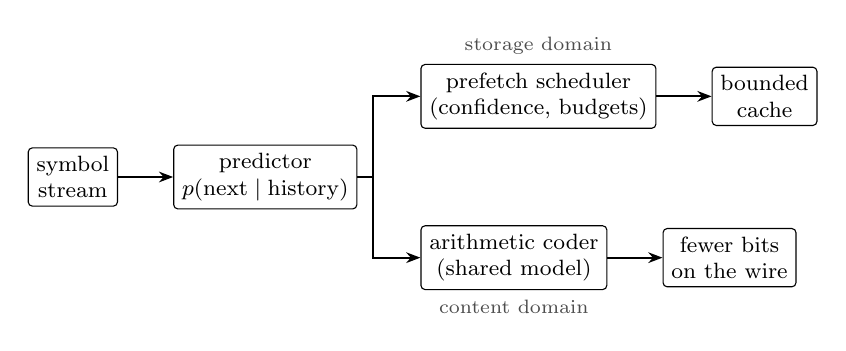
\begin{tikzpicture}[
  box/.style={draw, rounded corners=1.5pt, minimum height=7mm, align=center, font=\footnotesize, inner sep=3pt},
  arr/.style={-{Stealth[length=1.8mm]}, thick}]
\node[box] (obs) {symbol\\stream};
\node[box, right=7mm of obs] (pred) {predictor\\$p(\mathrm{next}\mid\mathrm{history})$};
\node[box, above right=2mm and 8mm of pred] (sched) {prefetch scheduler\\(confidence, budgets)};
\node[box, below right=2mm and 8mm of pred] (coder) {arithmetic coder\\(shared model)};
\node[box, right=7mm of sched] (cache) {bounded\\cache};
\node[box, right=7mm of coder] (wire) {fewer bits\\on the wire};
\draw[arr] (obs) -- (pred);
\draw[arr] (pred.east) -- ++(2mm,0) |- (sched.west);
\draw[arr] (pred.east) -- ++(2mm,0) |- (coder.west);
\draw[arr] (sched) -- (cache);
\draw[arr] (coder) -- (wire);
\node[font=\scriptsize, above=0mm of sched, text=black!70] {storage domain};
\node[font=\scriptsize, below=0mm of coder, text=black!70] {content domain};
\end{tikzpicture}}
\caption{One predictor feeds two consumers. The decoder in the content domain runs the same predictor on the data decoded so far, so only the model's surprises are transmitted.}
\label{fig:arch}
\end{figure}

\subsection{Storage testbed}\label{sec:storagebed}
The testbed has five modules: a byte-bounded cache (LRU or LFU, never exceeding its byte budget, returning stored values untouched), predictors, a scheduler, a trace-driven simulator, and a benchmark runner. Predictors are a sequential readahead, a stride detector, an order-$k$ Markov model with back-off (confidence is the product of transition probabilities along the predicted chain), and a clairvoyant oracle that reads the future from the trace as an upper bound. Frequency-based prediction is covered by LFU eviction rather than as a prefetcher, because it would mostly name items already cached. The scheduler acts only above a confidence threshold (0.4) and within caps on reads in flight (8) and bytes in flight (8\,MiB), and can back off when recent prefetches were wasted. The simulator models one FIFO storage device, so prefetch reads queue ahead of later demand reads, and a request for an item whose prefetch is still in flight waits only for the remainder (a late hit). Device parameters are nominal assumptions, not measurements: HDD 8\,ms and 150\,MB/s, SATA SSD 0.1\,ms and 500\,MB/s, NVMe 0.08\,ms and 3\,GB/s. Seven seeded workloads cover sequential, random, Zipf working-set, phased, recurring-routine and deep-learning epoch access, the last with and without reshuffling. The routines workload is our own construction to test the case where history repeats.

\subsection{Exact predictive codec}\label{sec:codec}
\cm{} is a deliberately small design in the lpaq lineage~\cite{mahoney2005}. A bitwise model predicts each bit from a direct-indexed context of the previous byte, hashed contexts of the previous 1, 2, 3, 4, 5, 6, 8 and 12 bytes, and a match model that follows the longest recent repeat. Each context slot holds an adaptive probability. A gated logistic mixer, with one weight set per partial byte, combines the stretched probabilities. A 32-bit binary arithmetic coder encodes each bit with the mixed probability~\cite{witten1987}.

\emph{Exactness.} All arithmetic is integer: probabilities are 12-bit, the logistic and its inverse are table lookups built from integers, and the mixer uses fixed-point weights. No floating point is used anywhere, so encoder and decoder compute identical probabilities on any machine, which a model shared between two computers requires and which floating-point neural models do not give by default. The container is one mode byte followed by either the model stream (an 8-byte length and the coded body) or the raw input. If the model stream is not smaller than the input, the encoder stores the input raw. This fallback is needed: on 50\,000 random bytes the bare model stream (small tables, in a unit test) was 3.5\,\% larger than the input, because high-order contexts learn noise. A decoder never reads past its input or writes past its declared output, and corrupt streams yield wrong bytes or an error, not a crash (tested by bit-flip fuzzing).

\emph{Tuning.} The mixer learning rate and counter limit were chosen by grid search on a separate tuning set of different files (stated in Section~\ref{sec:setup}), never on the test files. The chosen values changed mean bits per byte by under 1\,\% from the next best, so the result is not sensitive to them.

\subsection{When does coding win on the wire?}\label{sec:model}
Let $S$ be the file size, $B$ the bandwidth in bytes per second, $r$ the compression ratio, and $V_c$, $V_d$ the codec's compress and decompress throughput in bytes of original data per second. Sending raw takes $S/B$. We consider three cases. In the \emph{static} case the sender compressed the file in advance, so only the transfer and decompression are on the clock: $T=rS/B+S/V_d$. In the \emph{sequential} case compression, transfer and decompression run one after another. In the \emph{pipelined} case chunked streaming overlaps all three, an optimistic idealization where the slowest stage sets the time. Coding is faster than raw exactly when
\begin{equation}
B<(1-r)V_d,\quad B<\frac{1-r}{1/V_c+1/V_d},\quad B<\min(V_c,V_d)
\label{eq:be}
\end{equation}
respectively (the third requires $r<1$). Round-trip time and file size cancel. For two codecs, $a$ is faster than $c$ in the static case when
\begin{equation}
V_{d,a}>\frac{1}{(r_c-r_a)/B+1/V_{d,c}},
\label{eq:need}
\end{equation}
which gives the decoding speed a stronger but slower codec must reach to be worth using at a given bandwidth. The model ignores TCP dynamics, loss, parallel connections and CPU contention, and uses throughput measured on one machine.

\section{Experimental Setup}\label{sec:setup}
\emph{Corpus.} Table~\ref{tab:corpus} lists the ten test files, all real except one control. They come from the test machine (Python standard library, a system log, a compiled binary, JSON metadata, a JPEG) and from public test data (a bacterial genome and a viral genome). Files are capped at 1\,MiB. A separate tuning set, used only to choose \cm{} parameters, contains different files of the same kinds: odd-indexed standard-library sources, license text, an apt log, other JSON, a slice of another binary and a plasmid sequence. A manifest with SHA-256 hashes accompanies the corpus builder, because machine-local files differ between machines.

\begin{table}[t]
\caption{Test corpus (bytes). Three files are incompressible by construction or by prior compression.}
\label{tab:corpus}
\centering\scriptsize
\begin{tabular}{@{}lrl@{}}
\toprule
File & Bytes & Source \\
\midrule
source code & 1,048,576 & Python stdlib \texttt{*.py}, even-indexed \\
prose (docs) & 563,555 & Python language reference text \\
system log & 683,440 & \texttt{dpkg.log} \\
JSON & 1,048,576 & JSON metadata files \\
executable (ELF) & 1,023,032 & gcc driver binary \\
DNA, bacterial & 1,048,576 & \emph{B.\ fragilis} chromosome, FASTA \\
DNA, viral & 30,322 & SARS-CoV-2 genome, FASTA \\
gzip file & 1,048,576 & gzip of the bacterial genome \\
JPEG image & 292,349 & a library image \\
random bytes & 1,048,576 & seeded generator (control) \\
\bottomrule
\end{tabular}
\end{table}

\emph{Codecs.} gzip level 9, bzip2 level 9, xz preset 9e, zstd level 19, brotli quality 11 with a 16\,MiB window, and \cm. None uses a trained dictionary. Every output was decompressed and compared with the input by SHA-256, and the run aborts on any mismatch.

\emph{Measurement.} Compress and decompress times are the median of three wall-clock runs, single-threaded, on one machine: an Intel Xeon at 2.10\,GHz with two virtual CPUs and 7\,GiB of memory, Linux 6.18, Python 3.13, gcc 13.3 at \texttt{-O2} with no hand-written SIMD. Throughput is bytes of original data per second. It is machine-specific and should be read as relative. \cm{} allocates $8\times2^{22}$ four-byte slots (128\,MiB) per run, a fixed cost that dominates its time on very small files.

\section{Results}\label{sec:results}
\subsection{Compression}
Table~\ref{tab:bpb} and Fig.~\ref{fig:bpb} give compressed bits per input byte. \cm{} produced the smallest output on six of the seven compressible files, from 6.8\,\% smaller than the best of the five general codecs on the viral genome to 31.5\,\% smaller on the system log, with 10.6\,\% on source code and 11.3\,\% on prose. On the executable, xz was 5.2\,\% smaller. The gains are largest where text-like structure repeats at distance, consistent with the ablation below. On the random file and the gzip file, \cm{} stored the data raw at a cost of one byte, as did the other codecs within a fraction of a percent. The JPEG shrank by 9.5\,\% with \cm{} and by 9.0\,\% with the best general codec; we did not investigate whether this file is typical of JPEG data.

\begin{table}[t]
\caption{Compressed bits per input byte (lower is better; best in bold). $\Delta$ size compares \cm{} with the best of gzip, bzip2, xz, zstd and brotli ($-$ means smaller).}
\label{tab:bpb}
\centering\scriptsize
\begin{tabular}{@{}lrrrrr@{}}
\toprule
File & xz-9e & zstd-19 & brotli-11 & augur-cm & $\Delta$ size \\
\midrule
DNA, bacterial & 2.207 & 2.217 & 2.198 & \textbf{2.044} & $-$7.0\% \\
DNA, viral & 2.382 & 2.261 & 2.214 & \textbf{2.063} & $-$6.8\% \\
executable (ELF) & \textbf{2.389} & 2.555 & 2.446 & 2.512 & +5.2\% \\
JSON & 0.711 & 0.739 & 0.692 & \textbf{0.643} & $-$7.0\% \\
prose (docs) & 1.544 & 1.572 & 1.493 & \textbf{1.325} & $-$11.3\% \\
source code & 1.627 & 1.656 & 1.602 & \textbf{1.432} & $-$10.6\% \\
system log & 0.464 & 0.492 & 0.486 & \textbf{0.315} & $-$31.5\% \\
\midrule
gzip file & 8.001 & 8.000 & 8.000 & \textbf{8.000} & -- \\
JPEG image & 7.358 & 7.364 & 7.279 & \textbf{7.238} & -- \\
random bytes & 8.001 & 8.000 & 8.000 & \textbf{8.000} & -- \\
\bottomrule
\end{tabular}

\end{table}

\begin{figure}[t]
\centering
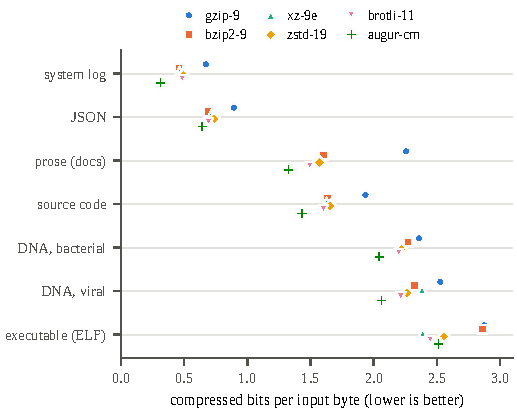
\includegraphics[width=\columnwidth]{figures/fig_bpb.pdf}
\caption{Bits per byte by file type and codec (lower is better). Marker shape identifies the codec; rows are offset slightly to separate overlapping points. The three incompressible files are in Table~\ref{tab:bpb}.}
\label{fig:bpb}
\end{figure}

\subsection{Speed}
Table~\ref{tab:speed} summarizes the compressible files by median. \cm{} has the lowest median size and by far the lowest speed: about 0.5\,MB/s in both directions, against 1090\,MB/s for zstd decompression and 386\,MB/s for brotli. Its compression speed is similar to brotli at quality 11, but brotli decompresses roughly 700 times faster. Context mixing is symmetric by nature, since the decoder repeats the encoder's work, while the strong dictionary codecs are asymmetric. On the 30\,kB viral genome \cm{} ran at only 0.24\,MB/s because of its fixed set-up cost.

\begin{table}[t]
\caption{Median over the seven compressible files.}
\label{tab:speed}
\centering\scriptsize
\begin{tabular}{@{}lrrr@{}}
\toprule
Codec & bits/byte & comp.\ MB/s & decomp.\ MB/s \\
\midrule
gzip-9 & 2.258 & 6.82 & 257 \\
bzip2-9 & 1.636 & 11.7 & 31.4 \\
xz-9e & 1.627 & 2.32 & 74.4 \\
zstd-19 & 1.656 & 2.49 & 1090 \\
brotli-11 & 1.602 & 0.50 & 386 \\
augur-cm & 1.432 & 0.52 & 0.52 \\
\bottomrule
\end{tabular}

\end{table}

\subsection{Time on the wire}\label{sec:wire}
Applying Eq.~(\ref{eq:be}) to the measured ratio and speed gives Table~\ref{tab:be}. Against sending raw, \cm{} wins on a static file below 2.7--5.9\,Mbit/s, so it does beat no compression on slow links. The comparison that matters is against the other codecs. Fig.~\ref{fig:time} shows the time to deliver 1\,MiB of source code: \cm{} is the fastest option only on very slow links, then flattens at about two seconds, the cost of decoding. Table~\ref{tab:winner} lists the fastest option per file type; at 0.5\,Mbit/s and above, \cm{} is never first. Its crossover (Table~\ref{tab:cross}) lies at 0.035--0.11\,Mbit/s on five of the six file types, and on the executable it never wins. To be the fastest option at 2\,Mbit/s, its decoding would have to be 16--53 times faster (Eq.~\ref{eq:need}), 72--214 times at 10\,Mbit/s and 321--822 times at 50\,Mbit/s. The advantage in bytes is real; the advantage in time is not, with this implementation, except under very scarce bandwidth.

\begin{table}[t]
\caption{Bandwidth (Mbit/s) below which \cm{} beats sending raw, by scenario, derived from measured ratio and speed (1\,MiB files; the 30\,kB file is excluded because set-up cost dominates it).}
\label{tab:be}
\centering\scriptsize
\begin{tabular}{@{}lrrr@{}}
\toprule
File & static & sequential & pipelined \\
\midrule
DNA, bacterial & 3.08 & 1.54 & 4.14 \\
executable (ELF) & 2.73 & 1.37 & 3.98 \\
JSON & 5.25 & 2.66 & 5.71 \\
prose (docs) & 3.27 & 1.64 & 3.92 \\
source code & 3.61 & 1.76 & 4.20 \\
system log & 5.88 & 2.96 & 6.13 \\
\bottomrule
\end{tabular}

\end{table}

\begin{figure}[t]
\centering
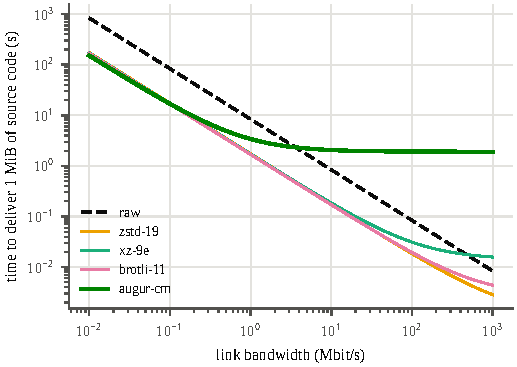
\includegraphics[width=\columnwidth]{figures/fig_time.pdf}
\caption{Static-case time to deliver 1\,MiB of source code versus link bandwidth, computed from measured ratios and speeds. Below about 0.1\,Mbit/s \cm{} is fastest; above it the other codecs win because they decode far faster.}
\label{fig:time}
\end{figure}

\begin{table}[t]
\caption{Fastest option (including raw) by link speed in Mbit/s, static case.}
\label{tab:winner}
\centering\scriptsize
\begin{tabular}{@{}lrrrrr@{}}
\toprule
File & 0.5 & 2 & 10 & 50 & 250 \\
\midrule
DNA, bacterial & brotli-11 & brotli-11 & zstd-19 & zstd-19 & zstd-19 \\
executable (ELF) & xz-9e & xz-9e & brotli-11 & zstd-19 & zstd-19 \\
JSON & brotli-11 & brotli-11 & brotli-11 & zstd-19 & zstd-19 \\
prose (docs) & brotli-11 & brotli-11 & brotli-11 & zstd-19 & zstd-19 \\
source code & brotli-11 & brotli-11 & brotli-11 & zstd-19 & zstd-19 \\
system log & bzip2-9 & xz-9e & brotli-11 & zstd-19 & zstd-19 \\
\bottomrule
\end{tabular}

\end{table}

\begin{table}[t]
\caption{Highest bandwidth at which \cm{} is still the fastest option (static case), and the factor by which its decoding must speed up to be fastest at 2, 10 and 50\,Mbit/s (Eq.~\ref{eq:need}).}
\label{tab:cross}
\centering\scriptsize
\begin{tabular}{@{}lrrrr@{}}
\toprule
File & fastest below & \multicolumn{3}{c}{speed-up needed at (Mbit/s)} \\
\cmidrule(l){3-5}
 & (Mbit/s) & 2 & 10 & 50 \\
\midrule
DNA, bacterial & 0.079 & 22$\times$ & 106$\times$ & 442$\times$ \\
executable (ELF) & never & -- & -- & 822$\times$ \\
JSON & 0.035 & 53$\times$ & 214$\times$ & 570$\times$ \\
prose (docs) & 0.081 & 23$\times$ & 105$\times$ & 348$\times$ \\
source code & 0.093 & 21$\times$ & 93$\times$ & 329$\times$ \\
system log & 0.11 & 16$\times$ & 72$\times$ & 321$\times$ \\
\bottomrule
\end{tabular}

\end{table}

\begin{table}[!t]
\caption{Ablation of \cm{}. $\Delta$ is the change in compressed size relative to the full model, as the mean and range over the five non-DNA files (source code, prose, log, JSON, executable); DNA is the bacterial genome. MB/s is the median compress throughput over the five files. Per-file values are in the repository.}
\label{tab:abl}
\centering\scriptsize
\begin{tabular}{@{}lrrrr@{}}
\toprule
Variant & mean $\Delta$ & range & DNA $\Delta$ & MB/s \\
\midrule
full model & -- & -- & -- & 0.53 \\
\midrule
no-match-model & +12.9\% & +4.0\% to +20.6\% & $-$0.1\% & 0.55 \\
orders$\leq$4 & +2.0\% & +0.3\% to +3.9\% & $-$0.3\% & 1.18 \\
orders$\leq$6 & +1.1\% & +0.0\% to +2.4\% & $-$0.2\% & 0.77 \\
order-2-only & +12.5\% & +3.2\% to +24.5\% & $-$0.2\% & 1.98 \\
table-bits=16 & +8.6\% & +6.1\% to +10.5\% & +0.1\% & 1.53 \\
table-bits=18 & +4.3\% & +3.7\% to +5.2\% & +0.0\% & 1.28 \\
table-bits=20 & +1.5\% & +1.2\% to +1.8\% & +0.0\% & 0.83 \\
table-bits=24 & $-$0.7\% & $-$1.0\% to $-$0.5\% & $-$0.1\% & 0.23 \\
\bottomrule
\end{tabular}

\end{table}

\subsection{Ablation}
Table~\ref{tab:abl} varies the model. Removing the match model costs 4.0--20.6\,\% on every non-DNA file, so it is the most valuable single component. Restricting contexts to orders 1--4 costs 0.3--3.9\,\% and more than doubles speed (1.18 versus 0.53\,MB/s); a single order-2 context costs 3.2--24.5\,\% but runs nearly four times faster. Orders 8 and 12 add up to 2.4\,\%. Table size matters: $2^{16}$ slots costs 6.1--10.5\,\%, while $2^{24}$ slots gains only 0.5--1.0\,\% at four times the memory (512\,MiB) and less than half the speed. DNA is nearly unaffected by every variant (within 0.3\,\%), which shows that byte-oriented contexts do not exploit its four-letter structure; a model built for that alphabet would likely do better, but we did not test one.

\begin{table}[!t]
\caption{Simulated speedup over LRU without prefetching (SATA SSD model, 3 seeds, median).}
\label{tab:storage}
\centering\scriptsize
\setlength{\tabcolsep}{3pt}
\begin{tabular}{@{}lrrrrrr@{}}
\toprule
Workload & sequential & stride & markov2 & markov2+gate & markov2-naive & oracle \\
\midrule
sequential & 1.38 & 1.38 & 1.00 & 1.00 & 1.00 & 1.38 \\
random & 1.00 & 1.00 & 1.00 & 1.00 & 0.52 & 1.28 \\
Zipf working set & 1.00 & 1.00 & 1.00 & 1.00 & 0.73 & 1.50 \\
phased & 1.06 & 1.13 & 0.99 & 1.02 & 0.69 & 1.30 \\
recurring routines & 1.00 & 1.00 & 1.08 & 1.10 & 1.05 & 1.28 \\
DL, reshuffled & 1.00 & 1.00 & 1.00 & 1.00 & 0.36 & 1.31 \\
DL, fixed order & 1.00 & 1.00 & 1.09 & 1.09 & 1.19 & 1.31 \\
\bottomrule
\end{tabular}

\end{table}

\subsection{Prefetching in simulated storage}\label{sec:storage}
Table~\ref{tab:storage} shows end-to-end speedup over an LRU cache without prefetching on the SATA SSD model, with the cache holding 5\,\% of the data, medians over three seeds. These results are simulated with nominal device parameters and are hypotheses for real-I/O tests, not measurements. Conventional readahead already captures sequential access (1.38$\times$), and the oracle shows that headroom exists elsewhere (1.28--1.50$\times$). A history-based Markov predictor gains only where history repeats: 1.08$\times$ on recurring routines (1.10$\times$ with the back-off gate) and 1.09$\times$ on fixed-order epochs. On random and reshuffled access it learns nothing, and accuracy does not equal speed: on the routines workload it reached 85\,\% accuracy but its tail latency was worse than the baseline because wasted prefetches queue ahead of real requests. Trusting a single observation is dangerous: the naive variant fell to 0.52$\times$ on random and 0.36$\times$ on reshuffled data, which is why the default requires two observations and smooths confidence, at the cost of learning more slowly (fixed-order epochs: 1.09$\times$ versus 1.19$\times$ over only three epochs). The outcome also depends on device speed relative to compute: with 100\,$\mu$s of compute per request, the Markov predictor on the routines workload gives 1.40$\times$ on the NVMe model but 0.89$\times$ on the HDD model, where reads are too slow for overlap to help and extra reads add contention.

\section{Discussion}
\emph{What the results support.} Prediction reliably saves bytes on predictable data, and a small model with no deep neural network already beats strong general codecs by 7--31\,\% on logs, text, code, JSON and DNA. It saves nothing on random or already-compressed data, and the fallback keeps the cost to one byte. Saving time is a separate question that depends on compute speed against link speed: with an unoptimized single-threaded model the answer is no above roughly 0.1\,Mbit/s. This also bears on the original motivation of helping people without fast connections: a slow link favors heavy compression, but the receiving device must run the model, so decode speed rather than model quality is the limiting factor.

\emph{What could change the answer.} Decoding would need to be 16--53 times faster to win at 2\,Mbit/s. Options we did not test are optimized and vectorized code, a GPU, splitting data into independently coded chunks to use several cores (at some cost in ratio), smaller or quantized neural predictors, and pretrained models shipped once and reused. Where bandwidth is metered rather than time-limited, the byte saving alone has value. For prefetching, server-side prediction paired with a client budget hint may avoid the waste seen in HTTP/2 push~\cite{chromium_push}, but we did not build or test it.

\emph{Threats to validity.} (i) All timing is from one shared virtual machine, three runs per cell; speed values are relative and ratios are unaffected. (ii) \cm{} is a small, unoptimized model; we did not run PAQ8, cmix or NNCP themselves, so we make no claim against the state of the art. (iii) Corpus files are small (at most 1\,MiB), include machine-local files, and cover few types; gains on other data may differ. (iv) Parameters were tuned on separate files, but all zstd and brotli settings are defaults for their levels and no dictionaries were trained, which would help small files. (v) The wire model is closed-form and ignores TCP and loss. (vi) Storage results are simulated with nominal devices, and the learned (neural) predictor of the original plan has not been built; only Markov and heuristic predictors were evaluated, so we make no claim about neural prefetching.

\section{Conclusion}
A model that predicts data can make it smaller, often substantially, and exactly. Whether that makes it faster depends on how cheap the prediction is relative to the time saved. In our measurements, a context-mixing codec beat five standard codecs on size for text-like data but would need decoding 16--53 times faster to win on time at 2\,Mbit/s, and simulated prefetching helped only where access history repeated. Next steps are real-I/O tests with cold-cache control, an optimized and parallel codec, a small neural byte predictor, and a network study of server-side prediction with client feedback.

\section*{Availability}
Code, corpus builder with hashes, raw measurements, and this paper's source are at \url{https://github.com/CygnusXl/Augur} (version 0.2.0).

\section*{Acknowledgment}
Experiment design, code and drafting were carried out with substantial assistance from Claude, an AI assistant from Anthropic. The author is responsible for the content.


\bibliographystyle{IEEEtran}
\bibliography{refs}

\end{document}
